\chapter{身長を予測する統計モデル}
\section{正規分布を組み入れた統計モデル}
日本人の$17$歳男性の身長を予測する統計モデルを構築する。この統計モデルは次の1-3から構成される。
\begin{quote}
    \begin{enumerate}[(1)]
    \item 独立同分布
    \item その分布は、正規分布
    \item 正規分布の母数(平均と分散)はそれぞれ$\mu,\sigma^2=5.7$。
    \end{enumerate}
\end{quote}

$\mu$を変数としたこの統計モデルを$M(\mu)$とする。
%数理統計学の知識を使うには、少なくとも$3$つので一つの統計モデルであると私は考えている。
およその平均値は日本にいれば母集団の分布をなんとなく知っているので、$\mu=171.1\mathrm{cm}$であると推測できる。
母集団のばらつき具合を意識することが少ないので、分散の値を決定することは難しい。
今回は、カンで$5.7$としました\footnote{統計データを覗き見した。分散を経験で推定できる人は少ないはずです。}。


\begin{SMbox}{なぜ正規分布を仮定できるのか}
  %\blindtext[5]
  数理統計学の本には、正規分布を前提にして書かれていることが多々あることから、科学において統計を利用するには、その前提が満たされる必要があるという考えがある。私も以前はそのように考えており、同様の考えにハマってしまう人は少なくない。

  \begin{rightbubbles}{bubblegreen}{Katsushi Kagaya}{./image/Twitter_logo_EPS/2021_Twitter_logo_blue.eps}
  学生のころ先生とデータについて議論していて(生物学分野です)「そもそもなぜ正規分布が仮定できるのか…」とおっしゃって二人でしばらく固まったことを思い出します。実現可能性の考え方から学ぶのが良いのかなと思います
      \begin{flushright} 
          \small	\url{https://twitter.com/katzkagaya/status/1209656621523058691}
      \end{flushright}    
  \end{rightbubbles}

  学問の世界において、分布関数に関する仮定が可能な理由についての認識は様々である。数学においては、仮定をして結論を導くことはよくある。数学から離れた科学の領域では、仮定することに対して妥当性や客観的であること要求していることもある。本書では、恣意的に考えたモデルを使って推測をしてみるという考えに基づいて、統計モデルを構築し、現象について推測を行う。
\end{SMbox}


\section{統計モデルによる推測}
$\mu=171.1$としたときの統計モデル$M(171.1)$を使って、身長に関する推測を行う。

\subsection{ $\circ\circ \mathrm{cm}$以下、$\diamond\diamond \mathrm{cm}$以上の人の割合}
まず、母集団に$180cm$以下、$180cm$以上の人の割合を推測する。正規分布関数を使い、$P(x>180)$を計算する。

\begin{lstlisting}
norm.cdf(180,171.1,5.7)
1-norm.cdf(180,171.1,5.7)
\end{lstlisting}
結果、 $P(x<180)=0.940$より、$P(x>180)=0.059$ということが分かります。
このことから、母集団から100人無作為抽出を行うと内$5-6$人程度は$180cm$以上であることが推測できる。

もう一つ、$160cm$以下の人割合を推測する。

\begin{lstlisting}
norm.cdf(160,171.1,5.7)
1-norm.cdf(160,171.1,5.7)
\end{lstlisting}
結果、$P(x<160)=0.059$、$P(x>160)=0.940$と推測できる。

$P(x<160)$と$P(x>180)$が極めて近い値でるのは、利用した正規分布は、母平均$\mu=171.1$を中心に、対称に分布する関数なので、$171.1$からおよそ$10cm$離れた$160cm$以下の人と$180cm$以上の人ではおよそ同じくらいの割合でいると推定される。
    
\subsection{擬似的に無作為を行うサンプリング}
$10$人分のデータをサンプリングしてみると、以下の数値が得られる。
$10$人を母集団から無作為抽出すると、およそこのようなデータが得られることがあると推測できる。

\begin{lstlisting}
168.575192 164.5988088 162.7027275 163.9689649 169.8187076 174.8851702 172.767133 165.0665034 175.7370453 163.0385381
\end{lstlisting}



\section{統計モデルの比較 1}
統計モデル$M(171.1)$による推測と実データを比較し、モデルがデータを推測できていることを確認する。
17歳男性の身長を無作為抽出して標本を得るには時間とお金がかかるので、公開されているデータ\footnote{ \url{https://www.e-stat.go.jp/dbview?sid=0003107092} }\footnote{\url{https://www.e-stat.go.jp/dbview?sid=0003037791}}を使う。
このデータは文部科学大臣があらかじめ指定した1410校の高校に在籍する生徒を対象にした標本である。

\begin{figure}
\begin{center}
    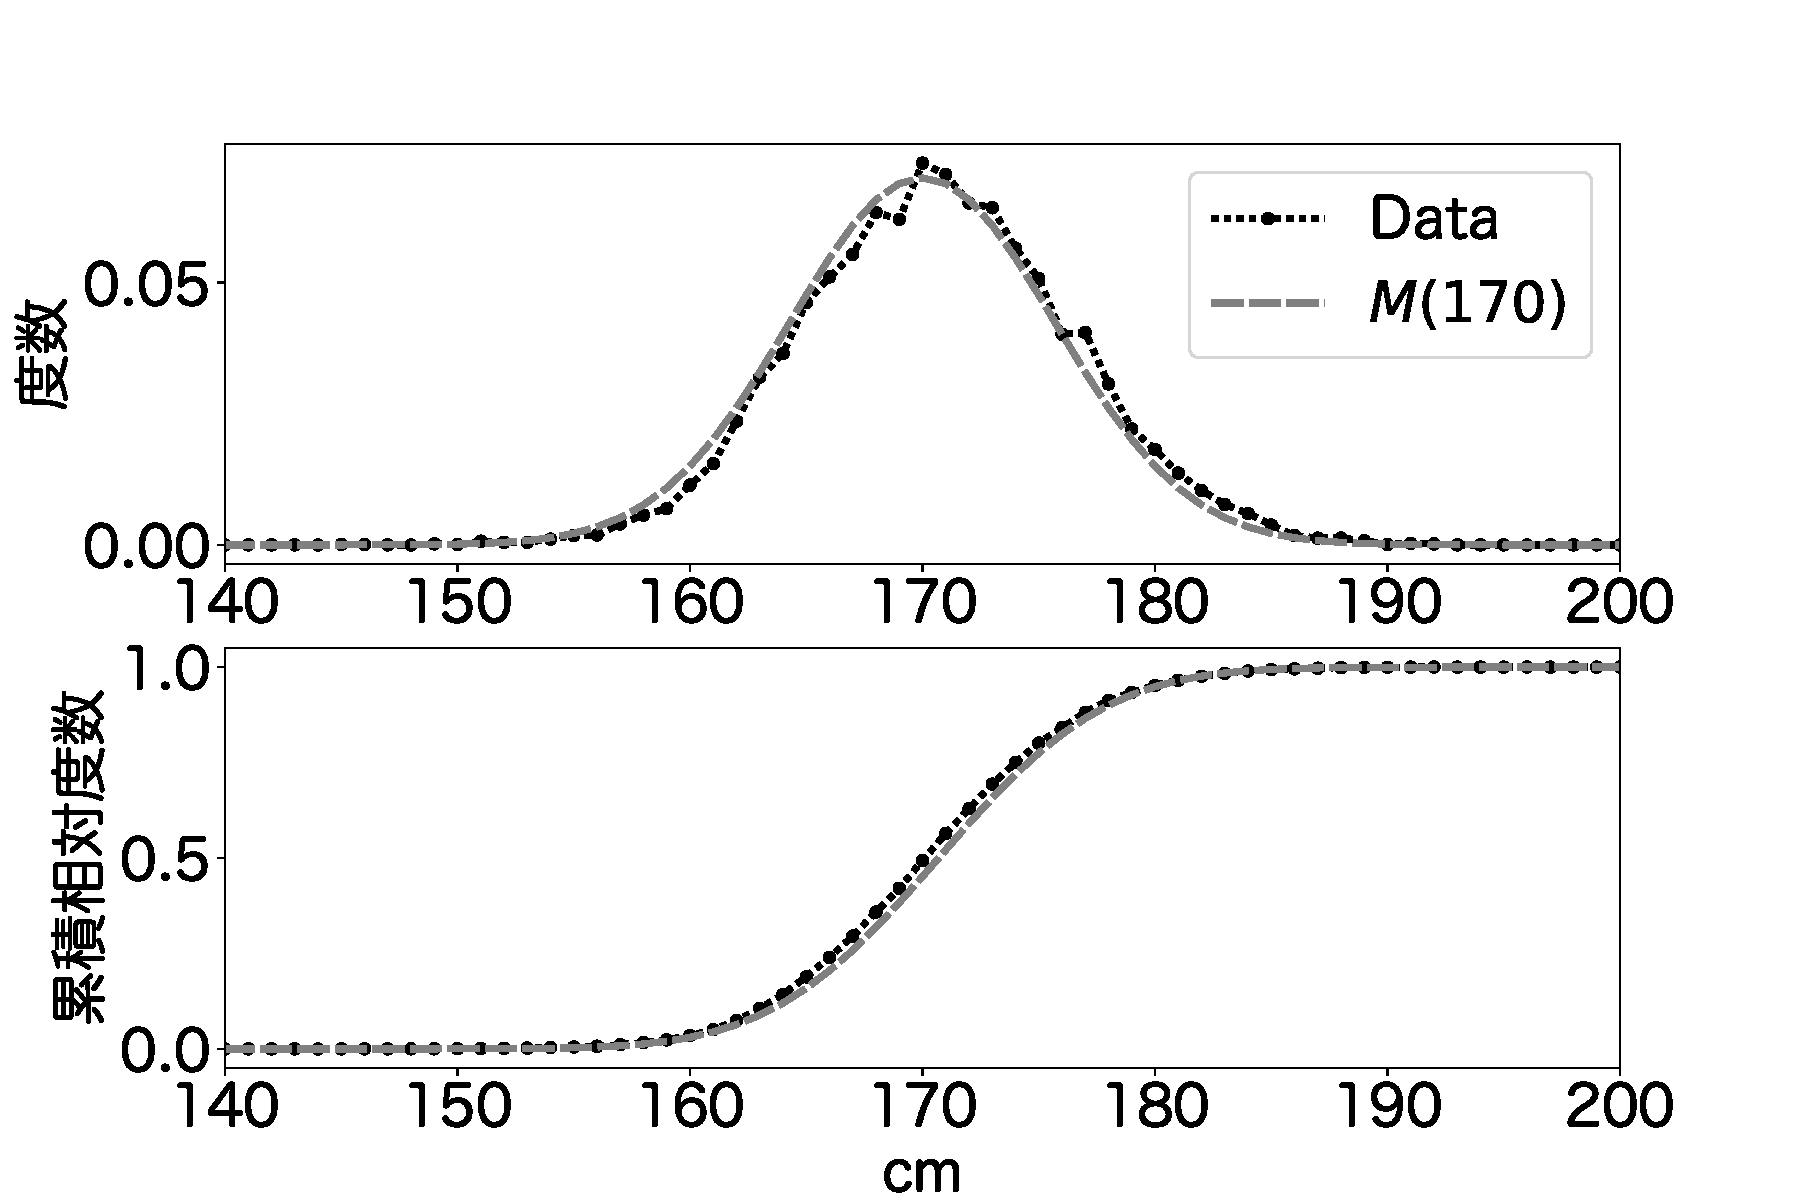
\includegraphics[width=15cm]{./image/03_/cm_data.pdf}
    \caption{17歳の男性から無作為抽出したデータ。上は、データと統計モデル$M(170)$の度数。下は、データと統計モデル$M(170)$の累積相対度数}
    \label{fig:real_height_men}
\end{center}
\end{figure}


\begin{SMbox}{$170cm$を少し超えた人が多いのは、不正(無作為抽出の手順に異常)があったから?}
\begin{quotation}
    「生物学上、グラフは曲線になっていなければならないが、169cmの部分はへこんでいる。これは先生や生徒による四捨五入で生まれるサバ読みの結果。身長が170cmなのか169cmなのかで気持ち的に違ってきますからね」と話すと、食料自給率や犯罪発生件数とは異なる微笑ましいサバ読みのトリックに、出演者一同、笑みを浮かべていた。\footnote{国民を欺く“統計のウソ” 知らないと怖い“統計トリック”を専門家が解説
    \url{https://times.abema.tv/articles/-/5640846} 2022/04/30確認}
\end{quotation}

このように、データが統計モデルに一致しないことから、データに不正な操作が加わっているという推測がされることがある。議論となっている身長のデータを観察してみる。
図\ref{fig:real_height_men}上を見ると、確かに、$170$を超えたあたりの度数は、$169$の度数よりも多い。
また、$170cm$以下のデータは統計モデルの度数よりも低く、$170cm$以上のデータは統計モデルの度数よりも大きい。一方で、図\ref{fig:real_height_men}下の累積相対度数を見ると、度数と同様の変異は少ないように見える。このようなデータと統計モデルの相違の原因は、不正な計測により生じたと断言できるのだろうか。

データとモデルの相違が生じる原因が、不正な計測だけではないことを確認する。
具体的には、データを統計モデルからサンプリングし、そのデータが統計モデルと一致するかを観察してみる(図\ref{fig:simulation_height_men})。図を見るとわかるように、サンプリングを行った場合、$168cm$付近で、度数が曲線よりも上にくる部分がある。また、$170cm$より小さいところでは、統計モデルよりもデータの度数が上にあり、$170cm$より大きなところでは、統計モデルより、データの度数が下にある。このように、統計モデルによりサンプリングし、統計モデルとサンプリングデータを比較した場合でも、ズレが生じる。これは、不正なモデルの予測とデータの間のズレが計測以外から生じることを示唆している。
%単純なズレだけを見たとしても、それが不正なのかは結論をつけることは難しい。


不正を見つけるには、次の経験が必要である。恣意的な操作を一切介入させない、かつ、無作為にデータを取得する条件のもと、得られたデータ、と同じ計測方法・同じ生徒において、教員が計測したデータこの二つのデータが一致しないならば不正な操作が加わったことが疑える。

データ解析をするには、常に、データを収集する手順が守られていないことを疑うことをするべきである。
例えば、髪の毛や靴などを履いる人がそうではない人と同じように計測をされると、平均値が大きくなる。身長の低い生徒に対してその傾向が高ければデータには歪みが生じやすくなる。計測を行なった先生方の疲れなども考慮すれば、データ収集の手順の誤りにより、データが偏ることもある。

データの収集には多大な労力がかかっている。誰かがどこかで腰を痛めながら高校生の身長を測る仕事をしていることは心に留めておくべきで、不正があったと主張するのは、彼らの仕事を低く評価しすぎではないだろうか。おそらく先生たちは、正確に計測できるように正確に手順を満たすように計測しているはずである。
不正を疑うならば、それなりに確証できる証拠を提示すべきである。具体的には、自分が手順を守って計測したデータと、先生が測ったときのデータにおいて、それらの間の差を示すべきである。



もう一つこの論者と私とで異なる点は、生物学データのグラフが曲線になるべきという点である。私は、推論のために統計モデルを利用しているので、統計モデルとデータが一致しない場合でも、推測に利用できると考え、統計モデルを利用する。一方で、この論者は、統計モデルとデータが一致すべきと考えている。言い換えれば、データが統計モデルに従うことを前提にする立場と、データを推論するために統計モデルを仮定すると言う立場がある。

\if 0 
$180cm$以上の割合についてはデータと一致していますが、$160cm$以下は、データと不一致です。この統計モデルで推測できていると考えても良いのでしょうか。
無作為抽出したときに得られるデータをできます。
ここで、$\mu=169.1$の統計モデル$M(\mu=169.1)$と、$\mu=180$の統計モデル$M(180)$を
標本から無作為抽出を行い、集計すると平均$169.1cm$程度であることがわかったとします。このとき統計モデル$M(169.1)$の推測は母集団の特徴をよく捉えているだろうか?
\fi 
\end{SMbox}

\begin{figure}
    \begin{center}
        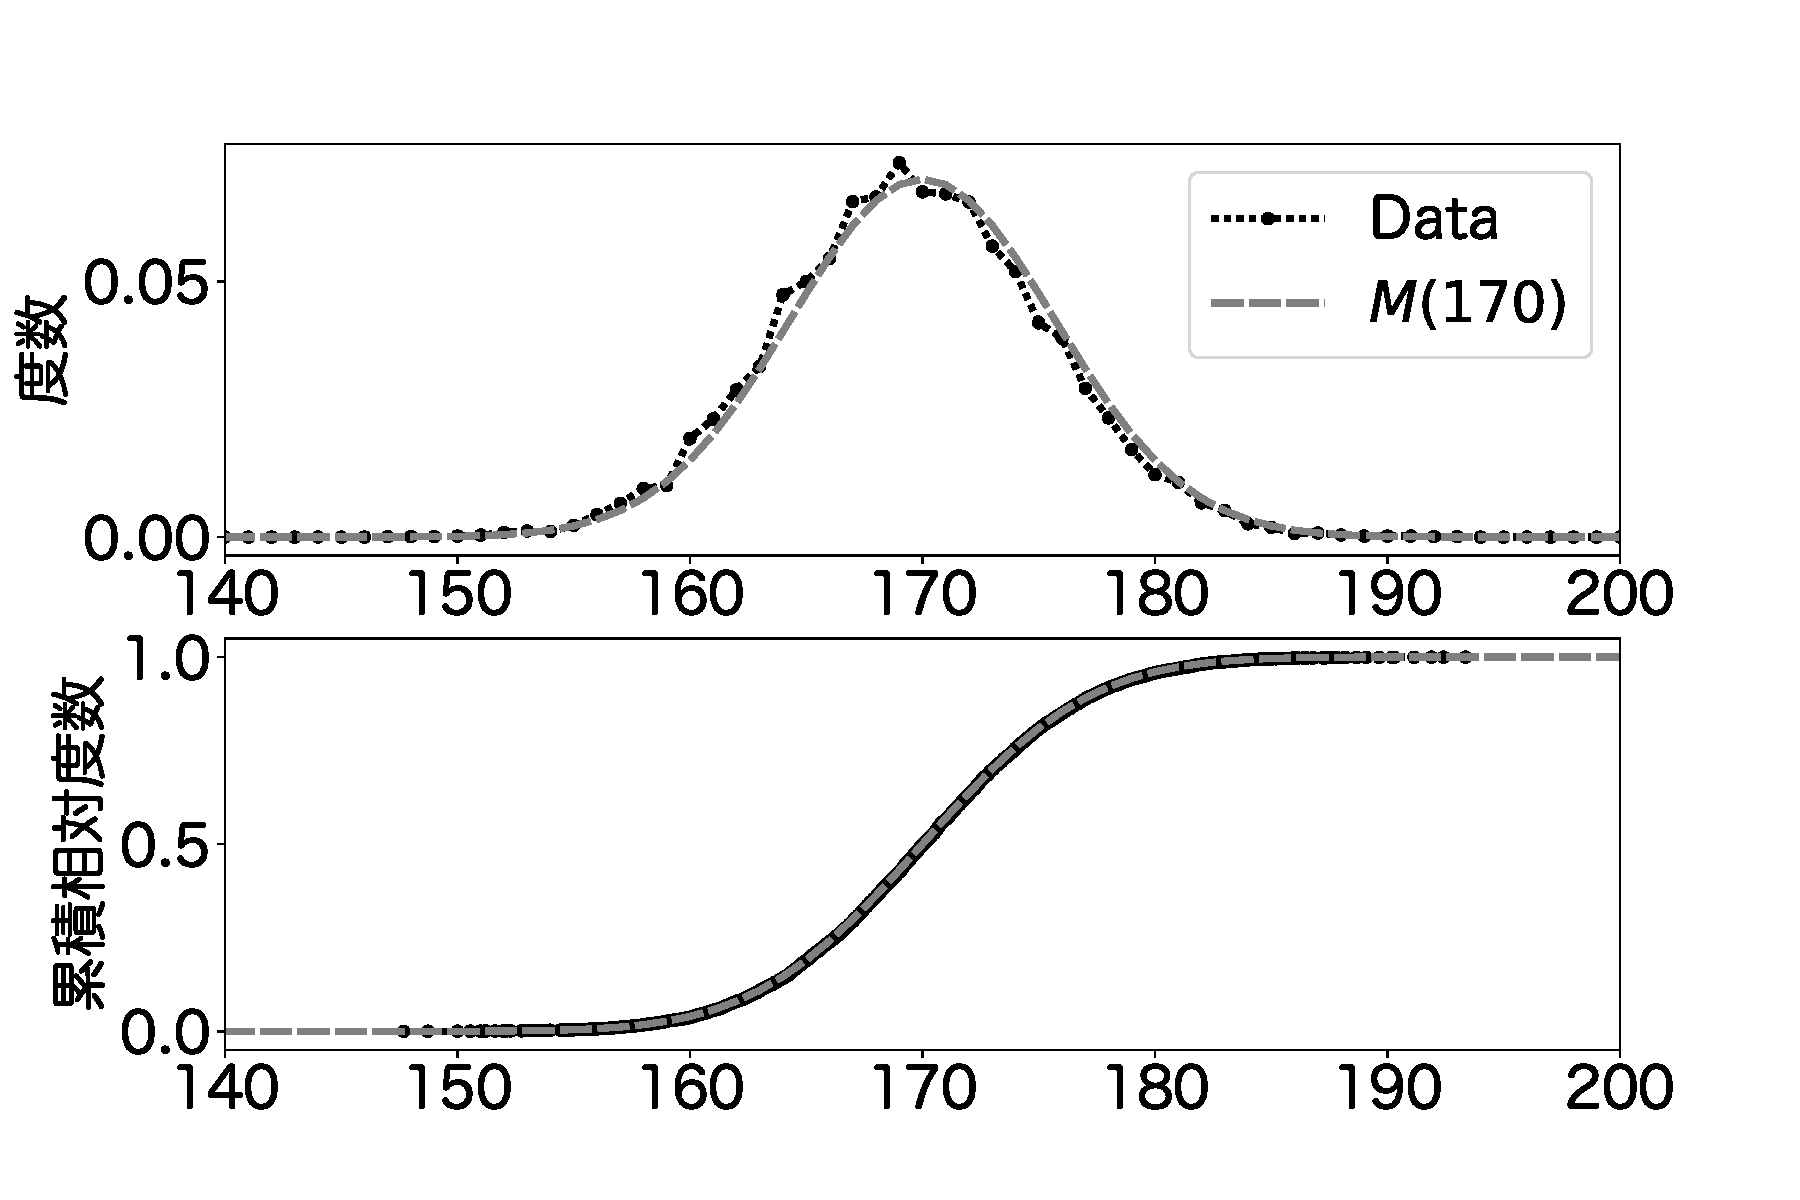
\includegraphics[width=15cm]{./image/03_/cm_data_simulation.pdf}
        \caption{上:正規分布を含む統計モデル$M(170)$によりサンプリングされたDataの頻度と、統計モデルの頻度。下:上と同じデータ・統計モデルの累積相対頻度}
        \label{fig:simulation_height_men}
    \end{center}
\end{figure}

\begin{SMbox}{軽いパンばかり買わされる}
ある国では、ある時期、パンを作るための道具、手順、材料が政府からパン屋に配布され、パン屋がパンを作ることになっていた。パンを焼くための型は、完成時に$1000g$になるように設計されており、手順を厳密に守り作ったパンは確かにおよそ$1000g$になっていた。どの季節に作っても手順を守りさえすれば、$1000g$になったのだ。
この材料、道具をパン屋が利用し、手順にそってパンを作れば、やはりパンはおよそ$1000g$になるはずである。

その国では、小麦の値段が高騰しており、支給された小麦をそのまま売った方が儲かるという状況になっていた。そんなとき、パンが$1000g$よりも軽いと感じた数学者が、数ヶ月にわたりパンの重量を計測していった。その結果、パンの重量は平均で$950g$となっており、本来の$1000g$よりも、軽いことがわかった。

このとき、パン屋が不正をしていると主張できる。
手順を踏めば平均で$1000g$になるパンが平均およそ$950$になったのは、パン屋が手順通りにパンを作っていないことを疑える。手順を守って作れば$1000g$になるという経験(データ)があるから疑うことができる。
%もしも、季節によってパンの重さが変化するものだったとするなら、$4$月には$1000g$だったものが$6$月には、$900g$になる可能性を排除できない。
\end{SMbox}


\subsection{サンプルサイズが大きい場合}

データと統計モデルを比較する。$180cm$以上の割合は、0.0642であり、モデル$M(171.1)$の推測値$P(x>180)=0.059$と数値が近い。
また$160cm$以下の割合は、$0.023$程度であり、統計モデルの推測値$P(x<160)=0.025$であり、やはり数値が近い。
%このように数学的フィクションである統計モデルを使うことで、現実に関する推測が可能になった。

ここまでは、$M(171.1)$を用いて、母集団を推測した。統計モデル$M(170)$の代わりに$M(168)$により推測を行うとデータとの一致具合を確かめる。$180cm$以上の人を推測すると$M(168)$では$P(x>180)=0.03$であり、統計モデル$M(171.1)$の推測$P(x>180)=0.059$よりもさらに実際の計測値$0.0642$と乖離している。
これは、$M(168)$では、ピークが平均値の$168$に移動するので、$180cm$を超える割合がさらに低くなるので、実際の数値から離れる。

一方で、$160$以下の人では、$M(168)$では、$P(x<160)=0.08$程であり、$M(171.1)$の推測値$P(x<160)=0.025$よりも、実際の数値$0.023$から離れている.
これも、$M(168)$では、ピークが$170$よりも小さな値になるので、$160cm$より小さい人の割合が大きくなるので、予測と実際のデータの不一致度が大きくなる(表\ref{table:data_type}にまとめておいた)。
このように、統計モデルの母数に応じて、現実の予測精度が変化する。

\begin{table}[hbtp]
    \caption{統計モデルとデータの比較}
    \label{table:data_type}
    \centering
    \begin{tabular}{lcc}
    %\hline
    統計モデル  & $P(x<160)$  & $P(x>180)$   \\
    \hline \hline
    データ &  0.023 &  0.0642\\
      %\hline \hline
    M(171.1) & 0.025 & 0.059  \\
    M(168) &  0.08 & 0.03 \\
      \hline
    \end{tabular}
  \end{table}


この統計モデルの予測の良さが分かったのは、無作為抽出を繰り返して、サンプルサイズを大きくしたときのデータの分布を得ていることによって、
そのデータとモデルとを比較をすることで、$M(171.1)$が$M(168)$より良い統計モデルであることを判別できた。

では、データが十分でない場合においても、推測とデータの一致を基準にして、より良い統計モデルを選ぶことはできるのでしょうか?

\subsection{サンプルサイズが小さい場合}
%\subsection{推測値とデータの比較}
母集団のことをほとんど知らない場合において、統計モデルとデータの比較はできるが、これを元に統計モデルが良いことを検討できない。
\if 0
母集団に関して次のことを知っていることにします。
\begin{itemize}
    \item 平均がおよそ$170cm$
    \item $160cm$の人や$180cm$の人と出会う確率は同じくらい($170cm$を中心に対象に分布している)
    \item 分散は5.7
\end{itemize}
\fi
サンプルサイズ10の標本が二つ得られたとします(実際には、コンピュータを使って正規分布からサンプリングした。このデータは母集団から無作為抽出したと考える)。標本は、次の通り。

\begin{lstlisting}
sample1 = [162.56944902, 178.42128764, 171.15286336, 172.2581195 , 160.21499345, 175.35072013, 173.17952774, 173.73301156, 179.52758126, 178.35924221]
\end{lstlisting}

\begin{table}[hbtp]
  \caption{統計モデルと小さいサンプルサイズの標本}
  \label{table:smalle_sample_size}
  \centering
  \begin{tabular}{lccc}
  %\hline
  統計モデル  & $P(x<160)$  & $P(x>180)$  & $\bar{X}$ \\
  \hline \hline
  標本1 &  0 &  0 & 172.8 \\
    %\hline \hline
  M(171.1) & 0.025 & 0.059  & 171.1 \\
  M(168) &  0.08 & 0.03 & 168\\
    \hline
  \end{tabular}
\end{table}
$180cm$以上の人は、$0$人、$160cm$以下の人も$0$人、どちらの統計モデルでも推測と一致しているかを推測できない[表\ref{table:smalle_sample_size}]。
標本平均$\bar{X}=172.8$であり、$M(170)$の母数$170$が$M(168)$の母数平均$168cm$でどちらも同じ程度の差である。
サンプルサイズが小さいときには、統計モデルの予測とデータを比較できないことがあるので、予測精度の良いモデルがどれかを決定できないことがある。


\if 0
sample2 = [164.04222157, 162.19052559, 172.03420244, 168.03580415, 176.73750537, 166.41177205, 165.27050656, 168.02537023, 176.18720054, 171.78005419]
\end{lstlisting}


\begin{table}[hbtp]
    \caption{統計モデルと小さいサンプルサイズの標本}
    \label{table:smalle_sample_size}
    \centering
    \begin{tabular}{lccc}
    %\hline
    統計モデル  & $P(x<160)$  & $P(x>180)$  & $\bar{X}$ \\
    \hline \hline
    標本1 &  0 &  0 & 172.8 \\
    標本2 &  0 &  0 & 169 \\
      %\hline \hline
    M(171.1) & 0.025 & 0.059  & 171.1 \\
    M(168) &  0.08 & 0.03 & 168\\
      \hline
    \end{tabular}
  \end{table}
どちらの標本でも

\fi
% また、標本の平均値と統計モデルの平均値でも標本が
% 仮説検定の枠組みでは、絶対にだめな統計モデルを明らかにします。

%\subsubsection{標本内の偏った値に注目}

%\section{統計モデルの比較 尤度・対数尤度}



\subsection{モデルの平均を含む信頼区間の個数}

実際に、$M(\mu=170)$を使って、$サンプルサイズを10$とし、標本を$100$個作ってみると、その分布は、図\ref{fig:confidence_interval_sample}Bのようになった。それぞれの標本に対してその信頼区間を描いたものが図\ref{fig:confidence_interval_sample}Aである。図Aの170cmのところにある縦の線は、統計モデル$M(\mu=170)$の母数平均である。
この170cmを跨いでいる信頼区間の個数はこの図では$96$個ある。コンピュータシミュレーションをするたびに毎回跨いでいる信頼区間の個数は変化するがおよそ95個である。このことは、信頼区間の定義から明らかである。


\begin{figure}
\begin{center}
    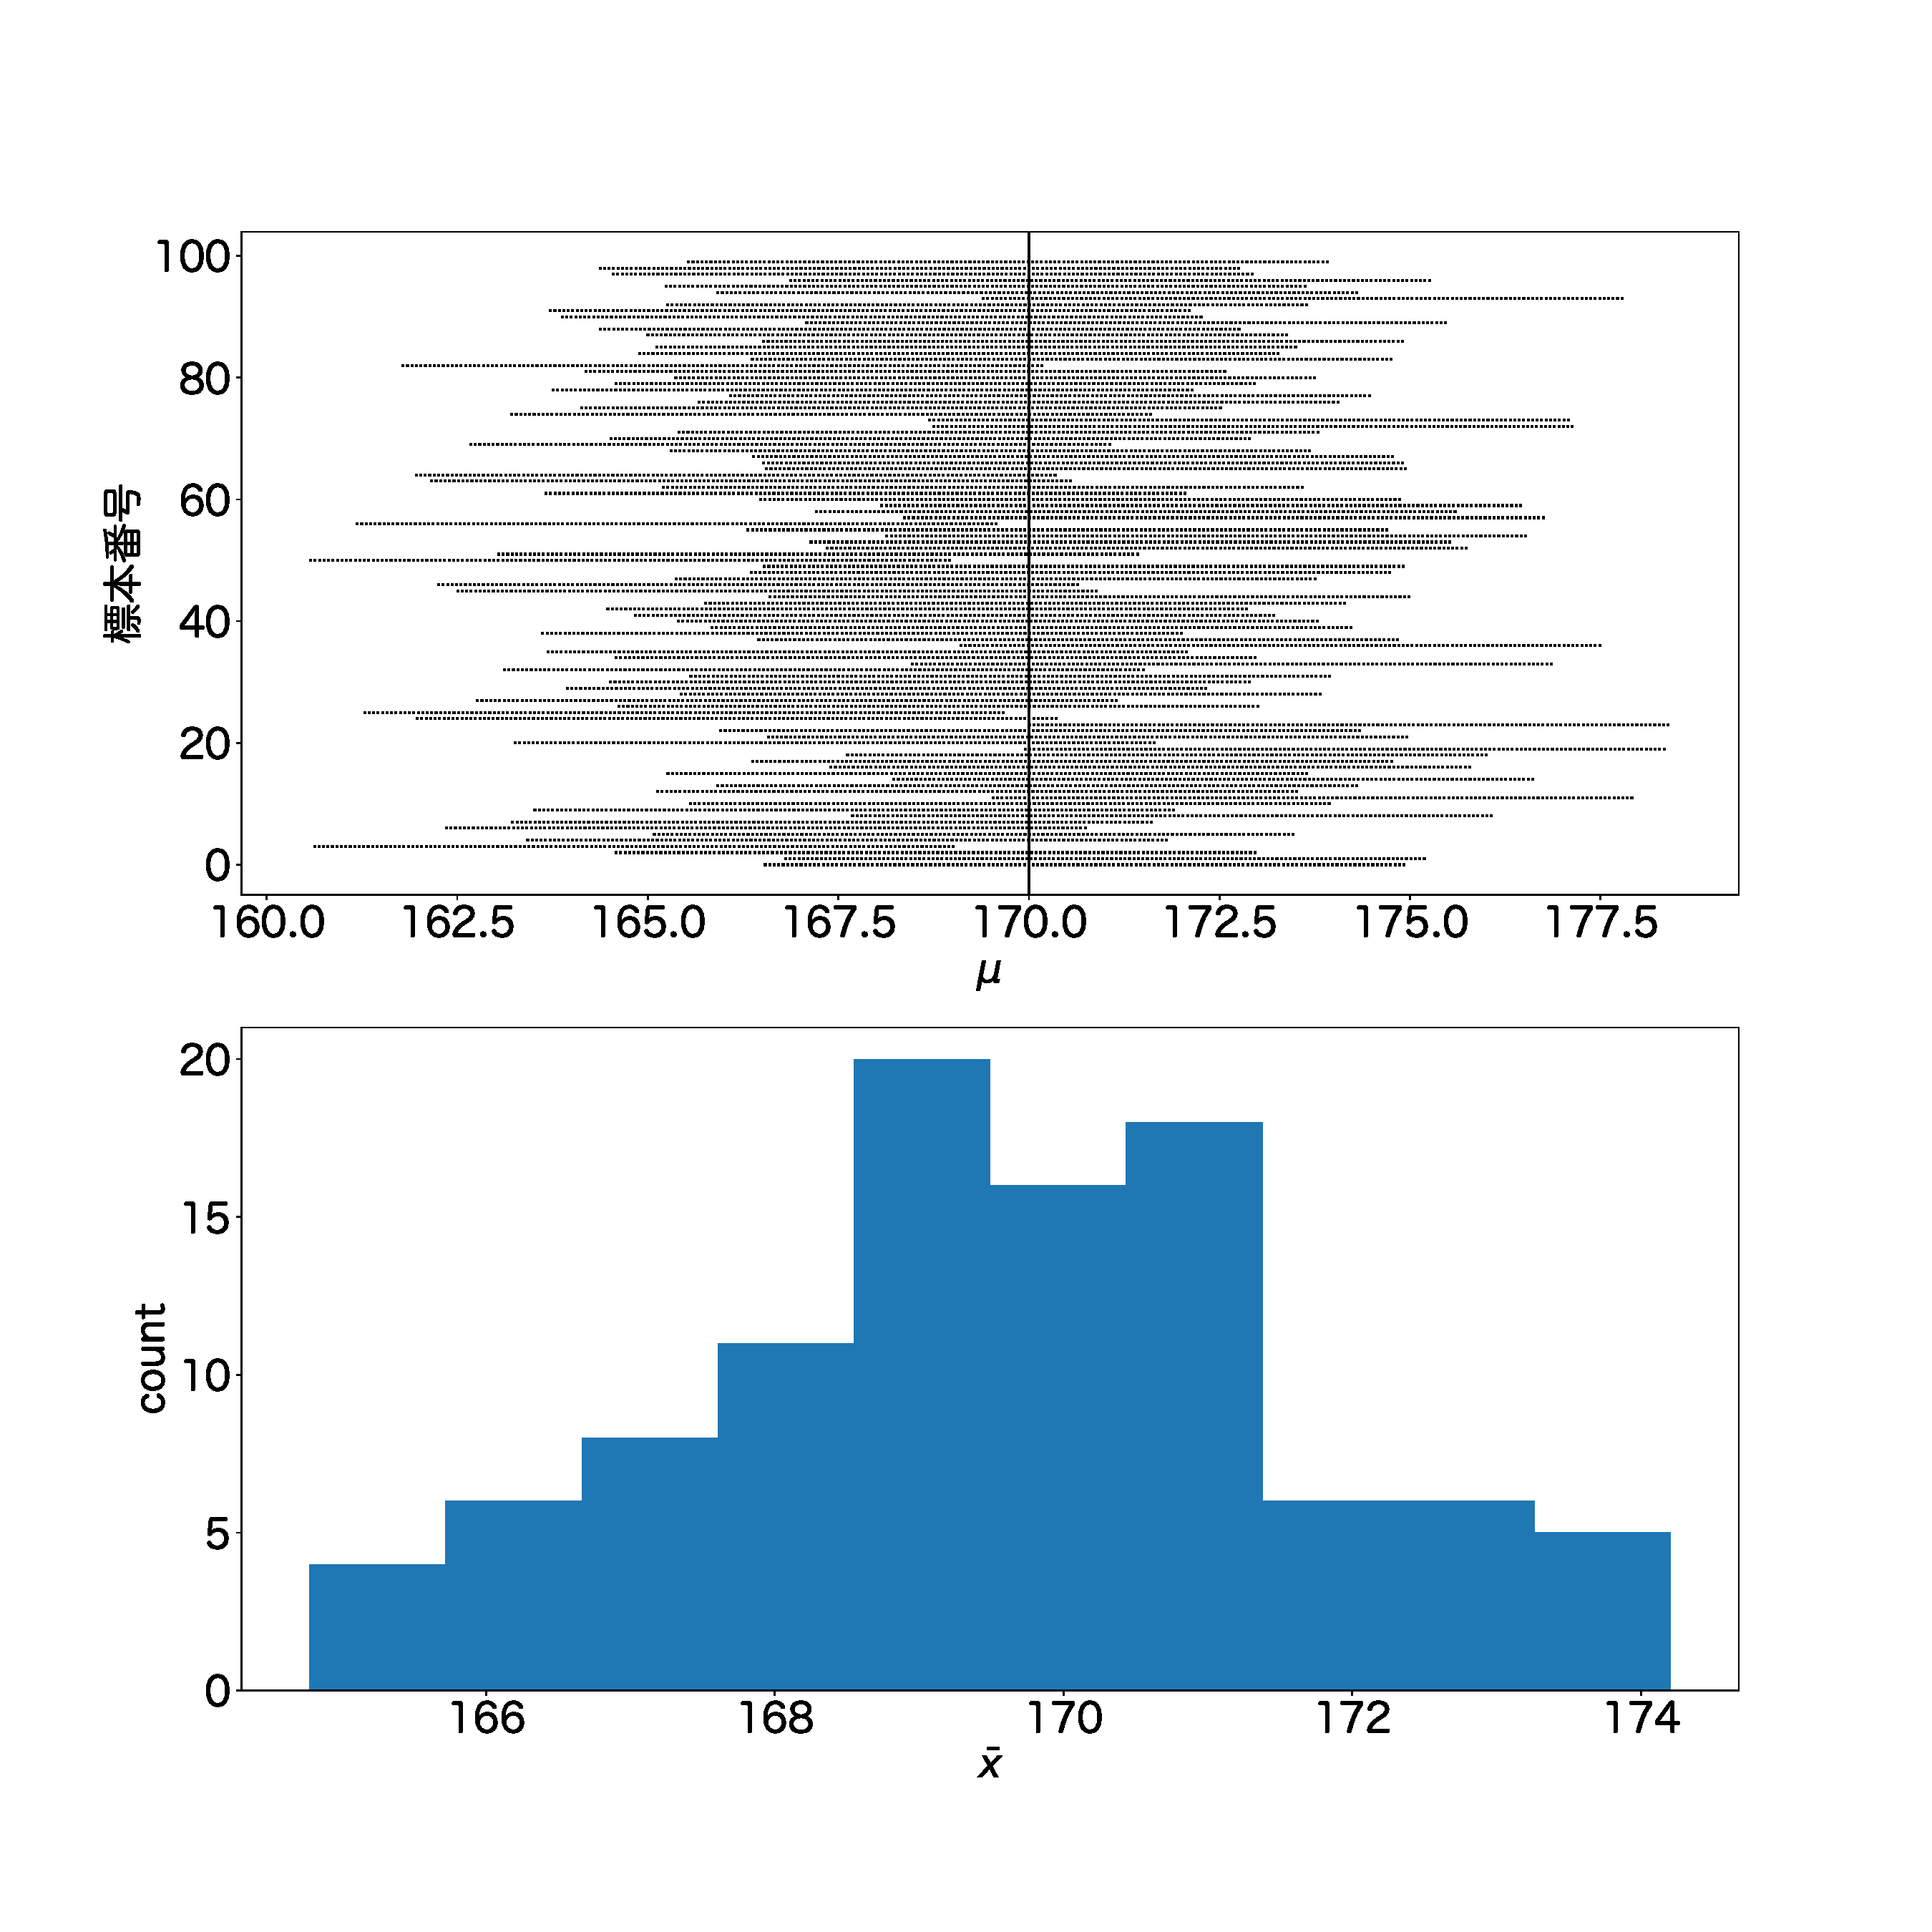
\includegraphics[width=15cm]{./image/03_/confidence_interval_model_count.pdf}
    \caption{(A)モデルから標本を得て、その標本から信頼区間を計算し、表示したもの。(B)標本平均の分布}
    \label{fig:confidence_interval_sample}
  \end{center}
\end{figure}


\begin{SMbox}{信頼区間は、データをたくさん取ったときに(サンプルサイズが同じ標本をたくさん集めたときに)、その範囲に真値が$95\%$の確率で含まれるの区間のこと}
信頼区間は、データをたくさん取ったときに、その範囲に真値が入る$95\%$の確率で含まれるの区間のこと\footnote{\url{https://www.slideshare.net/simizu706/ss-123679555}}。このように解説されることがある。
データを元に、統計モデルの母数を決定したときに、信頼区間が得られる。さらに計測を行い標本を作ると、標本の標本平均がこの信頼区間の間に含まれる確率が$95\%$であることを主張していると考えられる。

一般に、母集団が統計モデルにより、よく推測できるならば、無作為抽出の標本平均が$95\%$くらいの確率で信頼区間に含まれる。そうではないならば、$95\%$信頼区間にモデルの母数が含まれる確率は低く$95\%$とは異なる値をとる。

以上のことから、信頼区間は、データをたくさん取ったときに、その範囲に真値が$95\%$の確率で含まれるの区間のことという解釈はやめておいた方が良いと考えられる。
\end{SMbox}



\subsection{推測に利用できないと判定する}

\if 0
$N=1$では、$\bar{x}$が$154\sim185$あたりであれば、$M(170)$は棄却できない。$N=4$であれば、$\bar{x}$が$162\sim177$であれば、$M(170)$は棄却できない。$N=10$であれば、$\bar{x}$が$165\sim174$であれば、$M(170)$は棄却できない。
このようにサンプルサイズが増加することで、信頼区間が狭まり、棄却できるモデルの母数の範囲が狭まることがわかる。
\fi

\section{統計検定量によるモデルの評価}

\subsection{$Z(\bar{x},\mu)$以上の値が得られる確率}
$Z(\bar{x},\mu)\sim N(0,1)$により、$Z$以上の値が得られる確率も計算できます。つまり、
\begin{equation*}
    p = \varPhi(Z(\bar{x},\mu)>x)
\end{equation*}
です。$\bar{x}=172.4,\mu=168,\sigma^2=6.8,n=10$であれば、$Z(\bar{x},\mu)=2.04$であり、
$p=0.04$です。

\begin{lstlisting}
xbar = 172.4
mu = 168
sigma2 = 6.8**2
n=10
Z = np.sqrt(n)*(xbar-mu)/np.sqrt(sigma2)
print(Z)
p=1-norm.cdf(Z,0,1)
print(p*2)
\end{lstlisting}

\subsection{データの統計検定量と統計モデルの評価}
%母集団から無作為抽出したデータについて考えます。
無作為抽出によって得られた標本のサンプル$x_1,x_2,\cdots,x_n$について、その平均値を$\bar{x}$とする。
$M(\mu)$において、$\bar{x}$以上の値が得られる確率を計算する。
$\phi(z)$を標準正規分布とすると、$\phi(z>\frac{\sqrt{n}(\bar{x}-\mu)}{\sigma})$により求めることができる。
具体的な数値として、
$\bar{x}=172$なら、$\phi(z>\frac{\sqrt{n}(\bar{x}-\mu)}{\sigma}) = 0.289$であり、$\bar{x}=169$の場合、$\phi(z>\frac{\sqrt{n}(\bar{x}-\mu)}{\sigma}) = 0.133$である。$\phi(z>\frac{\sqrt{n}(\bar{x}-\mu)}{\sigma})$が$0.05$より大きい値を取ることから、統計モデル$M(\mu)$において、これらの観測値はよくある標本平均を得ている。$M(168)$でも同様に計算できる。

\begin{lstlisting}
    xbar = 172
    mu=171
    sigma = 5.7
    N=10
    c = np.sqrt(N)*(xbar-mu)/sigma
    1-norm.cdf(c,0,1)
\end{lstlisting}


%\section{データを元にした統計モデル}
%\subsection{最尤推定}

%\subsection{aaa}

%\subsection{推定した母数を持つモデルとそのほかのモデル}

